\section{Grundlagen}
\subsection{Schnittstelle}
Die Schnittstelle in der Informatik beschreibt sowohl den Bereich einer Software, der nach außen hin für andere Programme oder den Nutzer erreichbar ist, als auch eine eigenständig Anwendung, die zwei unabhängige Programme miteinander verbindet. Innerhalb einer Schnittstelle sind Funktionen vorgegeben, durch die der Nutzer mit der Software interagieren kann. Oftmals werden Schnittstellen für eine spezifische Anwendung entwickelt, um die Nutzung dieser Anwendung zu ermöglichen. Das Ziel einer Schnittstelle ist es, die Komplexität von bestehenden Programmen zu verringern. Der Satz der bereitgestellten Funktionen dient zur Vereinfachung der Bedienung komplizierter oder alter Programme. 
\footcite{sneed2006integrating}

Es wurden zwei Bereiche innerhalb der Schnittstelle entworfen. Der erste Bereich der Schnittstelle verbindet die Website mit dem Backend. Innerhalb des Backends wurde eine Schnittstelle in Form eines \ac{api} implementiert. Der zweite implementierte Bereich der Schnittstelle schließt das Backend mittels RabbitMQ an die einzelnen KI-Services an. In Kapitel 2.2 wird der Aufbau und die Funktionsweise der beiden Schnittstellen genauer erläutert.

\subsection{REST und RabbitMQ}
\subsubsection{Application Programming Interface}
Eine API ist eine Programmierschnittstelle, die dazu da ist, die Kommunikation zwischen einem Client, oder auch Anwender genannt, und einem Server durch festgelegte Funktionen zu regeln. Der Satz der verfügbaren Funktionen ist durch den Entwickler der API vorgegeben. Eine API sollte nach Möglichkeit selbsterklärend aufgebaut sein. \footcite{bloch2006design} Eine API dient dazu, dem Nutzer Daten bereitzustellen oder dem Server Daten zu senden.

In Abbildung 1 ist die Kommunikation zwischen einem Anwender und der API durch ein Sequenzdiagramm dargestellt. Jede Anfrage an die API findet durch den Aufruf des API Endpunkts durch einen \ac{url} statt. Hinter der Grund-URL wird die genaue Ressource innerhalb der API durch den Pfad in der URL angegeben. Jede dieser Funktionen, die über eine bestimmte URL erreichbar sind, kann mehrere Effekte haben. Der Effekt, den eine Funktion hat, ist durch die \ac{http} Methoden im groben Rahmen vorgegeben. Die Kommunikation zwischen API und Anwender geht immer vom Anwender aus. Die API kann den Anwender von sich aus nicht ansprechen. 

\begin{figure}[H]
  \centering
    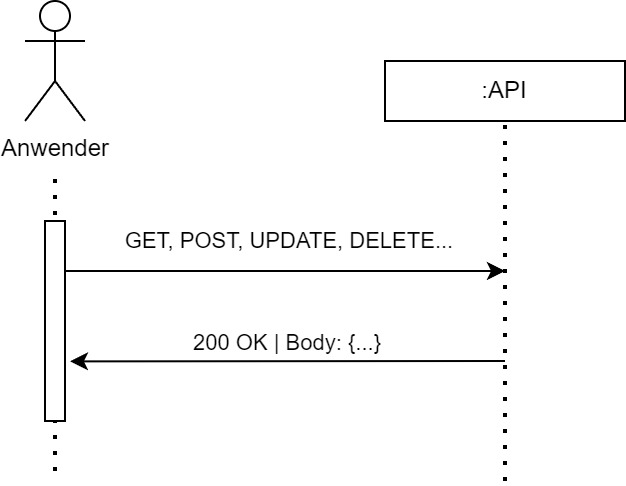
\includegraphics[width = 8cm]{bilder/APISequenzdiagramm}
    \caption{UML Sequenzdiagramm einer API}
\end{figure}

Der gesamte Satz der verfügbaren HTTP-Methoden lautet \texttt{GET, HEAD, POST, PUT, DELETE, CONNECT, OPTIONS, TRACE, PATCH}. Jede der Methoden hat eine bestimmte Aufgabe und bestimmte Rechte, die es vom Entwickler der API einzuhalten gilt.\footcite{mdn2022http} In der Bachelorarbeit werden die Funktionen \texttt{GET, POST} und \texttt{DELETE} verwendet. Routen der API, die mit einer \texttt{GET} Funktion aufgerufen werden, sollen lediglich Daten an den Nutzer zurückgeben, ohne Änderungen auf dem Server vorzunehmen. Wenn zweimal hintereinander die gleiche URL mit \texttt{GET} aufgerufen wird, sollte auch in beiden Fällen das gleiche Ergebnis von der API zurückgegeben werden.

Die \texttt{POST}-Methode liefert Daten vom Nutzer an den Server. Innerhalb des \texttt{POST}-Bodys können Daten im JSON-Format an die API gesendet werden. Neben dem JSON-Format gibt es auch noch weitere Möglichkeiten für Formate. Diese werden in der Bachelorarbeit jedoch nicht behandelt. API URLs, die mit einer \texttt{POST}-Methode aufgerufen werden, können Veränderungen auf dem Server auslösen. Dies kann Auswirkungen auf die Daten oder den Status des Servers haben, sodass andere Methoden eventuell davon beeinflusst werden. Ein beispielhafter Anwendungsfall für eine \texttt{POST}-Methode ist die Registrierung eines neuen Accounts auf einer Website. Dort werden innerhalb des Bodys der Benutzername und das Passwort an die API geschickt. Die API registriert den Account mit den erhaltenen Daten und gibt bei zukünftigen Aufrufen der URL mit den gleichen Daten eine Fehlermeldung zurück, dass der Benutzer bereits registriert ist.

Die \texttt{DELETE}-Methode entfernt eine Ressource unter der aufgerufenen URL. Sowohl bei \texttt{POST} als auch bei \texttt{DELETE}-Methoden ist darauf zu achten, dass der Nutzer die Route nur aufrufen kann, wenn er entsprechende Rechte zur Ausführung verfügt. Ansonsten könnte es zu unkontrollierten Daten- und Statusänderungen innerhalb der API kommen. 

Wie in Abbildung 1 zu sehen ist, gibt die API nicht nur die angeforderten Daten zurück, sondern auch einen Statuscode. Ein HTTP-Statuscode besteht aus drei Ziffern. In Tabelle 1 sind die grundlegenden Statuscodes aufgelistet.

\begin{table}[H]
\centering
\begin{tabular}{l|l}
\textbf{Statuscode} & \textbf{Bedeutung} \\
\hline
1xx & Informationen, nur unter HTTP 1.1 definiert \\
2xx & Request war erfolgreich (OK) \\
3xx & Die Ressource wurde verschoben \\
4xx & Die Eingabe war fehlerhaft \\
5xx & Der Server hatte einen Fehler \\
\end{tabular}
\caption{HTTP Statuscodes nach \cite{doglio2015pro}}
\end{table}

Die Statuscodes, die im Prototyp der Bachelorarbeit verwendet werden, sind Teil der häufiger genutzten Statuscodes für APIs. Der Statuscode \texttt{200:OK} ist der am häufigsten auftretende Statuscode. Dieser besagt, dass die Anfrage erfolgreich abgelaufen ist und das Ergebnis zurückgegeben werden konnte. Der Prototyp nutzt ein Authentifizierungssystem. Dadurch kann es dazu kommen, dass bei einer Anfrage mit fehlender Autorisierung der Statuscode \texttt{401:Unauthorized} zurückgegeben wird. Weitere Statuscodes, die häufiger auftreten können, sind \texttt{404:Not found}, \texttt{405:Method not allowed} und \texttt{500:Internal server error}. Bei einem Statuscode 404 wurde eine Route aufgerufen, die innerhalb der API nicht definiert ist. Bei dem Statuscode 405 wurde zwar eine vorhandene Route angesprochen, jedoch ist die genutzte HTTP-Methode nicht zulässig. Der letzte verwendete Statuscode 500 beschreibt eine fehlerhafte Ausführung der Anfrage. 

Die HTTP-Methoden und Statuscodes dienen dazu, die Entwicklung und Arbeit mit einer API für den Entwickler einfach zu gestalten. Wie die URLs der API aufgebaut sind und welche HTTP-Methoden wann verwendet werden, liegt jedoch vollständig beim Entwickler der API. Um APIs im Allgemeinen etwas zu vereinheitlichen und die Effekte der Funktionen innerhalb der API selbsterklärender werden zu lassen, wurde im Jahr 2000 von Roy Thomas Fielding ein Regelwerk namens \ac{rest} veröffentlicht.\footcite{fielding2000rest}

\subsubsection{Representational-State-Transfer}
REST ist ein Architekturstil, die den Aufbau der Kommunikation im World Wide Web. Der Representational-State-Transfer ist kein spezifischer Standard in der Softwareentwicklung. APIs, die versuchen, den Prinzipien dieses Architekturstils zu folgen, werden als \glqq REST-APIs\grqq{} oder \glqq RESTful-APIs\grqq bezeichnet. Diese bieten damit einen größtenteils standardisierten Weg, Daten zwischen Client und Server auszutauschen. \footcite{richards2006representational}

Innerhalb des REST-Frameworks sind mehrere Aspekte vorgegeben, die eine REST-API ausmachen. Drei der Aspekte sind Simplizität, Skalierbarkeit und Performance. Die Simplizität beschreibt einen allgemeinen, standardisierten Weg, wie der Aufbau und die Kommunikation mit der API ablaufen soll. Dies beinhaltet den Aufbau der Routen und damit der URL, wann Daten an die API geschickt werden sollen, sowie die Form der Daten, die zu versenden sind. 

Die Skalierbarkeit beschreibt das Konzept der beliebigen Erweiterung einer API. Das beinhaltet die Entwicklung der API als solche. Routen und damit Möglichkeiten, Daten von der API anzufordern oder Daten an die API zu senden, können während der Entwicklung einfach hinzugefügt und entfernt werden. Das Konzept der Skalierbarkeit beschreibt ebenfalls einen zustandslosen Aufbau der API. Durch die Zustandslosigkeit kann die API horizontal skaliert werden. Eine horizontale Skalierung beschreibt das Hinzufügen neuer Instanzen der API. Jede Instanz ist identisch aufgebaut und kann jede ankommende Anfrage alleinstehend beantworten. Die Anfragen, die an eine REST-API gestellt werden, müssen daher sämtliche für die Bearbeitung notwendigen Informationen bereitstellen.

Der letzte Aspekt des REST-Frameworks beschreibt die Performance. Eine REST-API implementiert ein System zum Zwischenspeichern, Caching gennant, von Responses. Wenn ein Client eine Anfrage mit der HTTP-Methode GET an die API schickt, wird die Antwort, die an den Client zurückgesendet wird, auf dem Server zwischengespeichert. Sollte ein oder mehrere Clients eine identische Anfrage an die API senden, wird das zwischengespeicherte Ergebnis zurückgegeben, statt die dahinter liegende Methode innerhalb der API neu auszuführen. Das ermöglicht eine hohe Performance, auch bei einer großen Anzahl von Anfragen.\footcite{masse2011rest}

\subsubsection{RabbitMQ}
Kommunikation ist für den Aufbau von komplexen Strukturen essenziell. Bei einer Kommunikation gibt es grundsätzlich zwei Beteiligte: Sender und Empfänger. Im Bereich der Software ist der Sender meist ein Client und der Empfänger ein Server, der öffentlich erreichbar ist. Der Client sendet eine Anfrage, der auch Request genannt wird, an den Server. Anschließend wartet der Client auf eine Antwort. Der Server erhält den Request und verarbeitet ihn. Es wird abhängig vom Request eine Antwort, die als Response bezeichnet wird, generiert und dem Client zurückgesendet. Der Client erhält die Response und schließt damit den Kommunikationsvorgang ab. Dieser Ablauf ist in Abbildung 2 visualisiert.

\begin{figure}[H]
  \centering
    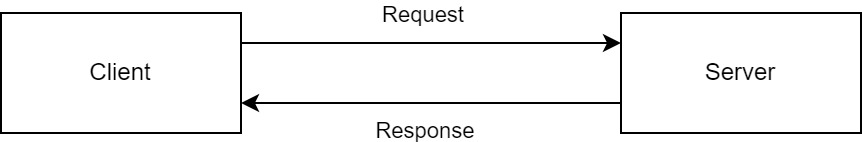
\includegraphics[width = 12cm]{bilder/Rabbit1}
    \caption{Grundlegende Kommunikation}
\end{figure}

Durch die synchrone Kommunikation sind Client und Server eng miteinander verbunden. Der Client erwartet eine Response von dem Server, an den er den Request geschickt hat. Die synchrone Kommunikation erhöht die Komplexität der Skalierung und Ausfallsicherheit.

Damit eine Kommunikation zwischen unabhängigen Programmen möglich wird, muss es einen Zwischendienst geben, der die Nachrichten von einem Programm zum anderen transportiert. Bei der Kommunikation zwischen einer Website und einer API wird das HTTP verwendet. Dieses stellt sicher, dass die die Nachrichten erfolgreich beim Empfänger ankommen. Sollte eine Nachricht nicht angekommen sein, hat der Absender die Möglichkeit, die Nachricht erneut zu schicken. Über HTTP wird automatisch eine erneute Anfrage geschickt, wenn keine Antwort vom Server zurückkam. Problematisch wird diese Herangehensweise, wenn die Antwortzeit sehr lang wird oder ungewiss ist, ob überhaupt eine Antwort kommen wird. Des Weiteren kann es zu Problemen führen, wenn sehr viele Nachrichten zur gleichen Zeit beim Server eintreffen. Der Server versucht sämtliche eingehenden Nachrichten gleichzeitig anzunehmen und zu verarbeiten. Dadurch entsteht eine sehr hohe temporäre Last. Sollte der Server seine Ressourcen, wie CPU oder RAM nicht dynamisch hochskalieren können, führen die eingehenden Anfragen zu einer Überlastung und damit zum Absturz des gesamten Servers.\footcite{hoque2015botnet} Um dies zu verhindern, muss ein Zwischendienst implementiert werden, der die eingehenden Nachrichten annimmt, zwischenspeichert und zum passenden Zeitpunkt weiterleitet, wenn der Server die erforderlichen Kapazitäten zum Verarbeiten einer neuen Anfrage hat.

RabbitMQ ist ein eine im Jahr 2007 veröffentlichte, nachrichtenorientierte Middleware, die eine Kommunikation zwischen zwei oder mehreren Programmen durch das \ac{amqp} ermöglicht. RabbitMQ implementiert einen Broker, der Nachrichten von mehreren Clients an mehrere Server vermitteln kann. Im Gegensatz zu einer direkten Kommunikation zwischen Client und Server wie bei HTTP, wird in RabbitMQ eine Queue implementiert, in der sämtliche Anfragen gesammelt werden.\footcite{JohanssonLovisa2020REBD} In Abbildung 3 ist die Kommunikation zwischen Client und Server mittels eines Brokers abgebildet.
 
\begin{figure}[H]
  \centering
    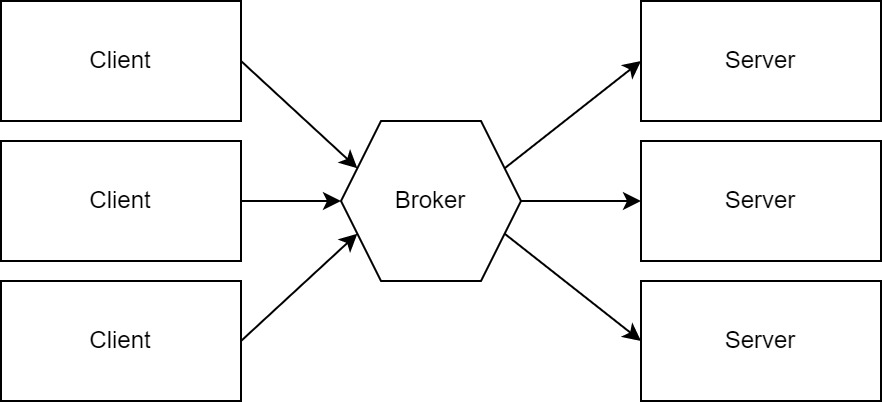
\includegraphics[width = 12cm]{bilder/Rabbit2}
    \caption{Kommunikation über einen Broker nach Dossot}
\end{figure}

Durch diese Herangehensweise wird eine asynchrone Kommunikation zwischen Client und Server ermöglicht. Sollte ein Server oder ein Client während seiner Laufzeit abstürzen, hat dies keine Auswirkungen auf die anderen Instanzen. Des Weiteren kann die Anzahl der Clients und Server, abhängig von der aktuellen Nutzlast, dynamisch hoch- und runterskaliert werden. Eine weitere Eigenschaft, die durch diese Architektur entsteht, ist, dass der Client keine Information darüber besitzen muss, wo sich der Server befindet, oder mit welcher Technologie er implementiert wurde. Solange der Server die Schnittstelle zum Broker implementiert, können die Nachrichten vom Client empfangen werden.\footcite{dossot2014rabbitmq}

Das AMQP ist ein offener Standard, der den Nachrichtenaustausch zwischen Produzent und Konsument regelt. AMQP definiert den gesamten Ablauf des Austausches. Innerhalb des Protokolls wird definiert, wie die \ac{tcp} Verbindung zwischen Client und Broker aufgebaut wird. Ebenfalls Bestandteil des Protokolls ist der softwareseitige Aufbau der Nachrichtenübermittlung. AMQP implementiert mehrere Konzepte, die auch im Prototyp verwendet wurden. Die folgende Aufteilung der Konzepte wurde durch Johansson und Dossot beschrieben.\footcite{JohanssonLovisa2020REBD}

Der Broker ist das grundlegende Konzept von AMQP. Er empfängt Nachrichten von einer Anwendung und leitet sie an eine andere Anwendung weiter.

Der Virtual-Host, genannt vhost, bietet eine Möglichkeit mit mehreren Anwendungen auf dem gleichen Broker zu arbeiten, jedoch ohne dass die Anwendungen Einfluss aufeinander nehmen können. Der vhost bietet eine logische Trennung der Anwendungen innerhalb der gleichen RabbitMQ Instanz.

Eine Connection beschreibt die physische Verbindung zwischen einer Anwendung und dem Broker. Die Verbindung zwischen Anwendung und Broker wird mittels TCP hergestellt. 

Ein Channel ist eine virtuelle Verbindung innerhalb einer Connection. Sendet ein Client eine Nachricht an einen Broker, wird dafür eine virtuelle Connection aufgebaut, statt jedes Mal eine neue TCP-Verbindung zu nutzen. Innerhalb einer Connection können mehrere Channels aufgebaut und genutzt werden. Dadurch können auch mehrere Anfragen über die gleiche TCP Verbindung abgearbeitet werden. 

Ein Exchange hat die Aufgabe, die Nachrichten zwischen Anwendung und Broker zu vermitteln. Der Exchange stellt sicher, dass die Nachrichten ankommen und in die richtige Queue geschrieben werden. In welcher Queue die Nachrichten landen, ist abhängig von den Regeln, die durch den Exchange Typen definiert werden.  

Eine Queue ist eine Datenstruktur, in der mehrere Operationen definiert werden. Die Queue fungiert als Warteschlange, in der Einträge gespeichert und in der Reihenfolge des Eingangs wieder ausgelesen werden. Sie funktioniert nach dem First In - First Out, kurz FIFO, Prinzip. Es wird eine \texttt{push} Operation definiert, mit der ein Eintrag an den Anfang der Warteschlange geschrieben wird. Des Weiteren gibt es eine \texttt{pop} Operation, die das älteste Element aus der FIFO-Queue ausliest und es aus der Warteschlange entfernt. Jeder Client kann Nachrichten in die Queue schreiben. Diese Nachrichten werden dort so lange gespeichert, bis sie von einem Dienst ausgelesen werden. 

Binding beschreibt eine virtuelle Verbindung zwischen einem Exchange und einer Queue innerhalb des Brokers. Diese Verbindung ermöglicht Nachrichtenfluss von einem Exchange zu einer Queue.

In Abbildung 4 sind die Konzepte von AMQP und deren Ablauf visualisiert.

\begin{figure}[H]
  \centering
    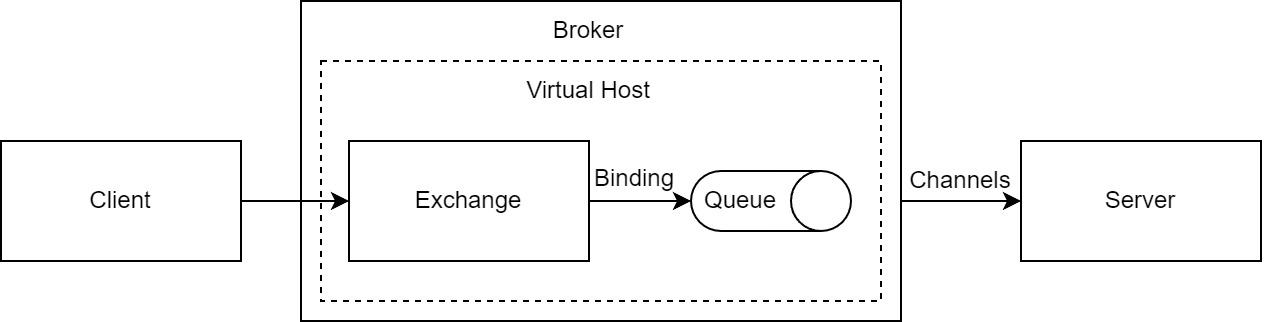
\includegraphics[width = 15cm]{bilder/Rabbit4}
    \caption{Darstellung der AMQP Konzepte nach Dossot}
\end{figure}

Die Middleware RabbitMQ wird im Prototyp für die Kommunikation zwischen der Flask API und den KI-Services genutzt. Sowohl das Backend, in dem die API implementiert ist, als auch die einzelnen KI-Services sind als Teil einer Microservice-Architektur implementiert. RabbitMQ wird als universelle Schnittstelle für die Kommunikation in der Microservice-Architektur verwendet. 

\subsection{Microservice-Architekturen}
Das Konzept von Microservices beschreibt die Unterteilung einer umfangreichen Anwendung in einzelne Teilanwendungen. Eine Teilanwendung wird dabei Microservice genannt. Die einzelnen Teilanwendungen sollen dabei untereinander kommunizieren können, um die Zusammenarbeit zu gewährleisten. Dazu nutzen die Teilanwendungen eine universelle Schnittstelle. Eine Anwendung soll nur eine Aufgabe erledigen. Der Umfang dieser Aufgabe ist nicht genauer definiert.\footcite{wolff2018microservices}

Die Idee von Microservices ist es, ein großes System in viele kleine einzelne Systeme aufzuteilen. Dadurch entsteht eine Modularisierung der einzelnen Services. Voneinander unabhängige Softwaremodule können im Gegensatz zu einem Softwaremonolithen unabhängig voneinander deployed werden. Dies ermöglicht es zur Laufzeit bestimmte Teile des Softwaresystems hoch- und runterzufahren. Ein Austausch von fehlerhaften Services oder das Dazuschalten von neuen Services bei mangelnder Leistung ist, während das Softwaresystem in einer Produktivumgebung genutzt wird, möglich.\footcite{newman2015microservices}

Jedes Teilsystem kann einzeln deployed werden. Dadurch kann die Verfügbarkeit des gesamten Systems gewährleistet werden, auch wenn bestimmte Bereiche der Software aktualisiert oder verändert werden müssen. Bei einem Monolithen müsste für jede Änderung am System die gesamte Anwendung heruntergefahren und neugestartet werden.  

Microservices sind voneinander unabhängige Programme und damit auch eigenständige Prozesse. Die Technologie, mit der ein Service implementiert wird, ist nicht durch die allgemeine Architektur oder das System vorgegeben. Jeder Service kann in der für ihn passenden Technologie und Programmiersprache entwickelt werden. 

Da die Technologien der Services unabhängig voneinander sind, muss es eine gemeinsame Schnittstelle zur Kommunikation geben. Über diese Schnittstelle werden Daten und Information ausgetauscht, die die jeweiligen Services zum Bearbeiten ihrer Aufgaben benötigen. Die Kommunikation im Prototyp wird mit RabbitMQ implementiert. 

\subsection{Künstliche Intelligenz}
Der Begriff KI beschreibt eine Software, die das Ziel hat, typisch menschliche Aufgaben, wie Sehen, Hören und Verstehen von Kontext abzubilden.\footcite{gorz2010handbuch} 
KIs benötigen eine große Menge an Daten als Grundlage, mit denen sie trainiert werden können. Ein nicht trainiertes KI-Modell kann nicht viel mehr als zufällige Entscheidungen treffen. Erst durch das Training bekommen die Entscheidungen der KI eine Struktur. Nachdem eine KI für ihren bestimmten Einsatzzweck mit den entsprechenden Daten trainiert wurde, kann sie verwendet werden. Die Verwendung einer KI folgt den Grundprinzipien eines normalen Algorithmus. Es wird ein Input angenommen, wie beispielsweise ein Text oder ein Bild. Dieser wird durch die KI analysiert und in eine für die KI verständliche Form gebracht.\footcite{hamet2017artificial} Diese Form ist im Falle des Prototyps ein 512-dimensionaler Vektor. Anschließend generiert die KI einen Output. Dieser kann das Endergebnis der Anfrage sein oder für weitere Verarbeitungsschritte genutzt werden.

KIs können von Grund auf selbst entwickelt und trainiert werden. Die Anwendungszwecke einer KI überschneiden sich jedoch oftmals mit bereits vorhandenen Modellen, die es frei oder gegen eine Nutzungsgebühr auf dem Markt gibt. Wenn eine fertig trainierte KI genutzt werden kann, spart dies Entwicklungszeit und Ressourcen. Die vortrainierten KIs werden jedoch meist als Blackbox angeboten. Eine Blackbox ist ein geschlossener Raum, der eine Eingabe annimmt und eine Ausgabe produziert, ohne dass der Nutzer der Blackbox sehen kann, wie der Algorithmus funktioniert, der zu der Ausgabe führt.  

Ein KI-Service beschreibt eine Implementierung einer solchen Blackbox. Ein KI-Service ist ein alleinstehendes Programm, das die Aufgabe hat, Nachrichten anzunehmen, sie zu transformieren, zu analysieren und anschließend ein oder mehrere Ergebnisse zurückzugeben. 

Um die Nachrichten empfangen und die Ergebnisse zurücksenden zu können, muss in jedem Service eine Schnittstelle implementiert sein, über die die Nachrichten empfangen werden können. Innerhalb des Prototyps wird in den einzelnen KI-Services RabbitMQ als Schnittstelle genutzt.

Im Prototyp zur Anbindung von austauschbaren Datenquellen an KI-Algorithmen ist ein Service zur Textähnlichkeitssuche implementiert. Dieser nutzt das \ac{bert}-Modell von Google. Dieser Service ermöglicht die semantische Suche in einer Datenbank. Nicht-KI-gestützte Textsuchalgorithmen können in einer Datenbank lediglich nach übereinstimmenden Wörtern oder Wortteilen suchen. Wenn ein Nutzer sämtliche Einträge zu einem bestimmten Thema aus der Datenbank herausfiltern möchte, muss die passenden Schlüsselwörter kennen, die in den Datenbankeinträgen vorhanden sind. Sucht man in einer Datenbank beispielsweise nach \glqq JavaScript\grqq{} und es gibt nur Artikel, die die Abkürzung \glqq JS\grqq{} beinhalten, liefert die Suche keine Ergebnisse. Eine gewisse Textähnlichkeit kann erreicht werden, wenn zum Beispiel Leerzeichen oder Groß/Kleinschreibung ignoriert werden. 

Eine Textänlichkeitssuche, die mittels KI durchgeführt wird, kann zu einer Anfrage wie \glqq JavaScript\grqq{} deutlich mehr Ergebnisse liefern. Sie ist nicht durch die in der Suche angegebenen Zeichen beschränkt, sondern versucht den Inhalt der Anfrage zu verstehen. Anschließend kann in der Datenbank nach inhaltlich ähnlichen Artikeln gesucht werden, die zur Anfrage passen. Der \glqq verstandene\grqq{} Satz, der für die Suche in der Datenbank genutzt wird, ist abhängig vom verwendeten KI-Modell. Für die Textähnlichkeitssuche im Prototyp wird das BERT Modell von Google verwendet, um die Anfrage in einen 512-dimensionalen Vektor zu konvertieren. Jede Dimension des Vektors wirkt sich auf die Interpretation des Vektors aus. Der Vektor wird daher auch als \glqq dense vector\grqq{}, oder auch dichter Vektor bezeichnet. Damit die Suche über den Vektor funktioniert, wird ein zweiter Vektor benötigt, mit dem der, durch die Suchanfrage erzeugte, Vektor verglichen werden kann. Jeder Eintrag in der Datenbank muss daher einmalig mit dem gleichen KI-Modell analysiert werden. Der jeweils erzeugte Vektor wird in der Datenbank abgespeichert, um ihn für kommende Suchanfragen nutzen zu können.

Der Grundsatz des KI-Modells ist es, dass zwei Sätze, die inhaltlich ähnlich sind, auch zwei ähnliche Vektoren besitzen. Vektoren sind ähnlich, wenn der Abstand der beiden gering und die Richtung ähnlich ist.\footcite{rahutomo2012semantic} Diese Abstandsberechnung kann in der Elasticsearch Datenbank seit Version 7.3, welche am 31.07.2019 veröffentlicht wurde, automatisch durchgeführt werden. 

\subsection{Verwendete Werkzeuge}
\subsubsection{Python API mit Flask}
%Implementierung der Rest api durch Flask
Python ist eine um 1991 von Guido van Rossum entwickelte Programmiersprache. Bei der Entwicklung von Python wurde ein besonderer Fokus auf die Lesbarkeit von Code gesetzt. Dank der simplifizierten Syntax im Vergleich zu anderen höheren Programmiersprachen wie Java oder C\#, ist Python auch in Bereichen, wie in der Mathematik oder der Wissenschaft ein häufig genutztes Werkzeug. Python bietet ebenfalls die Möglichkeit, von anderen Entwicklern bereitgestellte Bibliotheken in das eigene Projekt zu integrieren.\footcite{python2021python} 

Flask ist eine der verfügbaren Bibliotheken, die ein Framework für die Implementierung einer webbasierten API bereitstellt. Eine API dient dazu, Funktionen und Routen zu definieren, um die Kommunikation zwischen dem Frontend und dem Backend herzustellen. Das Flask-Framework ist im Gegensatz zu anderen Frameworks sehr klein. Dies ermöglicht ein schnelles aufsetzen und entwickeln. Da Flask nur die nötigsten Grundlagen für eine API mitliefert, ist der Code besser lesbar und damit für andere Entwickler besser wartbar.\footcite{grinberg2018flask} 

Die Flask-API wird für die Anbindung des Frontends an die Datenbank, sowie die Anbindung an die Kommunikationsschnittstelle von RabbitMQ verwendet. Sie nimmt die Daten oder die Eingaben des Nutzers entgegen und vermittelt sie an den richtigen Dienst, damit sie von einer KI-Schnittstelle ausgewertet werden können. Anschließend kann die API angefragt werden, ob es bereits Antworten von einer KI zu der vorher geschickten Anfrage gab. Falls die API die Auswertung der KI erhalten hat, wird diese für das Frontend bereitgestellt, um sie dort anzeigen zu können.  

\subsubsection{REDIS und MySQL-Datenbanken}
Redis ist eine In-Memory Key-Value-Datenbank. Im Gegensatz zu \ac{rdbms} wie MySQL oder PostgreSQL werden in Redis keine festen Tabellenstrukturen hinterlegt. Redis gehört damit zur Kategorie der NoSQL-Datenbanken (Not Only SQL). Key-Value-Stores sind kein Ersatz für eine relationale Datenbank, bieten aber für bestimmte Bereiche große Vorteile. Durch das Fehlen von komplexen Strukturen innerhalb der Datenbank kann Redis Anfragen weitaus schneller als andere Datenbanksysteme bearbeiten. Da Redis im \ac{ram} ausgeführt wird,  werden die Daten grundsätzlich nicht persistent gespeichert. ACID (Atomicity, Consistency, Durability and Isolation) Konformität wird mit Redis ebenfalls nicht gewährleistet. Für den Einsatzzweck als Cache in einer Cloud-Umgebung ist Redis allerdings sehr gut geeignet. \footcite{paksula2010persisting}

Innerhalb des durch Redis implementierten Key-Value-Stores werden sämtliche relevanten Daten gespeichert, die ein Nutzer während seiner Benutzung der Software produziert. Dort werden ebenfalls die Zwischenergebnisse abgespeichert, die die KI während der Analyse erstellt.
%
%\subsection{MySQL Datenbank für Services und Logs}
MySQL ist ein um 1995 erschienenes Open-Source RDBMS. MySQL ist eines der weitverbreitetsten und schnellsten Datenbanksysteme in seiner Kategorie. \footcite{dubois2008mysql}

In relationalen Datenbanken werden Daten strukturiert in Tabellenform abgespeichert. Einzelne Tabellen können Verlinkungen und Referenzen auf andere Tabellen haben, damit die Zusammengehörigkeit der Daten beschrieben werden kann, ohne Daten redundant speichern zu müssen. In MySQL, wie auch anderen RDBMS, werden Tabellenstrukturen und Daten persistent abgespeichert. In-Memory-Datenbanken wie Redis können Daten über Umwege auch persistent speichern, jedoch müssen dafür größere Anpassung an der Konfiguration von Redis vorgenommen werden.

Das RDBMS MySQL wird u. a. für die Speicherung der Logs, die der Flask-Server während der Verarbeitung von Requests oder Nachrichten an die KI produziert, verwendet. Ein weiterer Einsatzzweck der MySQL-Datenbank ist die Speicherung der im System registrieren KI-Services. Ein Dienst kann über die Flask-API im System registriert oder deregistriert werden. Das Frontend kann im Anschluss eine Auflistung der verfügbaren Services beim Backend anfragen.

\subsubsection{Angular Frontend}
Eine Website wird üblicherweise mit \ac{html} und JavaScript erstellt. Um eine moderne Website zu entwickeln, die ihren Inhalt nicht beim ersten Aufrufen lädt, sondern erst dann, wenn er benötigt wird, müssen Konzepte wie \ac{ajax} verwendet werden. Angular ist ein von Google entwickeltes und gepflegtes Open Source-Framework, zur Vereinfachung des Entwickelns von komplexen webbasierten Anwendungen. Angular bietet im Gegensatz zu anderen Webframeworks wie React und Vue.js eine vollumfängliche Bibliothek, mit der nahezu sämtliche Aspekte in der Web-Entwicklung abgedeckt werden können.\footcite{moiseev2018angular}

In Angular wird die Programmiersprache TypeScript verwendet. Diese ist eine Erweiterung der Programmiersprache JavaScript und implementiert Konzepte wie feste Typisierung von Variablen. Weitere Konzepte wie Dependency-Injection oder die Trennung von \ac{bl} und \ac{ui} ermöglichen eine schnelle Entwicklung von komplexen Systemen. 

Das Frontend wird für die Ein- und Ausgabe der Daten verwendet. Der Nutzer kann auf der Webseite seine Suchanfrage in ein Textfeld schreiben und anschließend auf den Server hochladen. Im nächsten Schritt wird die Möglichkeit bereitgestellt, die eingegebenen Daten automatisiert zu bearbeiten und zu manipulieren. Im gleichen Zug wird die Eingabe des Nutzers in ein für die KI verständliches Format konvertiert. Im letzten Schritt schickt der Nutzer die Anfrage an das Backend, mit der Analyse der Eingabe zu beginnen. Das Frontend fängt daraufhin an, beim Backend in regelmäßigen Abständen nach Antworten der KI zu fragen. Antworten werden in einer Liste visualisiert.

\subsubsection{Logging durch Grafana}
Grafana ist ein von Torkel Ödegaard in 2014 entwickeltes Open-Source-Datenvisualisierungsprogramm. Grafana kann zeitbasierte Daten durch verschiedene Arten von Grafen und Diagrammen anzeigen.\footcite{chakraborty2021grafana}

Eines der möglichen Panels für ein Dashbaord ist das Log-Panel. Dort werden die Log Nachrichten aus einer Datenbank angezeigt und mit einer Farbe, abhängig vom Schweregrad markiert. Als Datenquelle können u. a. zeitbasierte Datenbanken z. B. InfluxDB und Prometheus oder RDBMS wie MySQL verwendet werden.

Im implementierten Prototyp wurde eine MySQL verwendet, in der die zu loggende Nachricht, der Schweregrad, der Zeitstempel und die User-\ac{id} gespeichert werden. Diese Daten werden verwendet, um die Logs im Log-Panel von Grafana chronologisch anzeigen zu lassen.

\subsubsection{Deployment über Docker}
Docker ist eine Software zur Isolierung von Anwendungen mithilfe von Containervirtualisierung. Ein Container beschreibt eine in sich geschlossene Umgebung, in der ein Programm ausgeführt werden kann. Die benötigten Dateien, Parameter und Umgebungsvariablen werden beim Starten des Containers mitgegeben. Damit wird sichergestellt, dass ein innerhalb eines Docker-Container ausgeführten Programms sich in jeder Umgebung gleich verhält. Hierdurch wird die Unabhängigkeit vom Host-Betriebsystem gewährleistet. Im Gegensatz zu einer \ac{vm} muss für die Ausführung eines Docker-Containers kein komplettes Betriebssystem virtualisiert werden. Das Hochfahren einzelner Container ist schneller und ressourcenschonender als die Implementierung einzelner VMs.\footcite{anderson2015docker} Des Weiteren können über das Docker-Compose-Plugin mehrere Container gleichzeitig hochgefahren werden, sodass mit einer einzigen Kommandozeileneingabe eine komplette Softwarearchitektur hochgefahren werden kann.

Docker wird für das Deployment der einzelnen Komponenten des Prototyps verwendet. Für Redis, MySQL, RabbitMQ, Grafana und Elasticsearch können die benötigten Images, die eine Bauanleitung darstellen, aus dem Docker-Hub heruntergeladen und genutzt werden. In einem Docker-Image sind sämtliche für die Ausführung des Programms benötigten Dateien gepackt. Docker-Hub ist eine Plattform zur Verteilung von offiziellen Docker-Images, von der automatisch die Images runtergeladen werden, die lokal nicht vorhanden sind.

Für das Angular-Frontend und das Flask-Backend müssen die Images manuell gebaut werden, bevor sie als Container gestartet werden können. Dafür bietet Docker sogenannte Docker-Files an, in der die benötigten Konfigurationen hinterlegt werden.

